% Created 2014-12-17 Wed 16:24
\documentclass[11pt]{template/openetcs_report}
\usepackage{fixltx2e}
\usepackage{graphicx}
\usepackage{longtable}
\usepackage{float}
\usepackage{wrapfig}
\usepackage{rotating}
\usepackage[normalem]{ulem}
\usepackage{amsmath}
\usepackage{textcomp}
\usepackage{marvosym}
\usepackage{wasysym}
\usepackage{amssymb}
\usepackage{hyperref}
\tolerance=1000
\usepackage{todonotes}
\usepackage{pdfpages}
\hypersetup{
  pdfkeywords={},
  pdfsubject={},
  linkbordercolor 	= {1 1 1},
  pdfcreator={Emacs 24.3.1 (Org mode 8.2.4)}}
%===========================
% Graphicpath
%===========================
\graphicspath{{./template/}{.}{./images/}}
%===========================
% Todo note margin
%===========================
\setlength{\marginparwidth}{7em}
%\let\oldmarginpar\marginpar
%\renewcommand\marginpar[1]{\-\oldmarginpar[\raggedleft\footnotesize #1]%
%{\raggedright\footnotesize #1}}
%===========================


\begin{document}
\frontmatter
\project{openETCS}


%assign a report number here
\reportnum{OETCS/WP7/07.3.5}

%define your workpackage here
\wp{Work-Package 7: ``Toolchain''}

%set a title here
\title{OpenETCS Roadmap}

%set a subtitle here
%\subtitle{}

%set the date of the report here


\date{\today}
\title{Traceability Architecture in OpenETCS}
\subtitle{WP7 Proposition}
%define a list of authors and their affiliation here

\creatorname{Cécile Braunstein}
\creatoraffil{University Bremen}
\techassessorname{}
\techassessoraffil{}

\qualityassessorname{}
\qualityassessoraffil{}

\approvalname{}
\approvalaffil{}
\author{Cecile Braunstein}
\affiliation{University Bremen}

\author{Moritz Dorka}
\affiliation{DB}


% define the coverart
\coverart[width=350pt]{openETCS_EUPL}

%define the type of report
\reporttype{OpenETCS : Position Paper on traceability}


\begin{abstract}
%define an abstract here
This document presents  apropostion to the tool chain traceability
architecture.
\end{abstract}


\maketitle
\tableofcontents

\newpage
%=============================

% The actual document starts below this line
%=============================
%Start here
%=============================
% Document Managment
%=============================
\chapter{Document Information}

\begin{tabular}{|p{4.4cm}|p{8.7cm}|}
\hline
\multicolumn{2}{|c|}{Document information} \\
\hline
Work Package &  WP7  \\
Deliverable ID or doc. ref. & O7.3.5\\
\hline
Document title &Traceability Architecture in OpenETCS \\
Document version & 00.02 \\
Document authors (org.)  & Cécile Braunstein (Uni.Bremen) \\
\hline
\end{tabular}

\begin{tabular}{|p{4.4cm}|p{8.7cm}|}
\hline
\multicolumn{2}{|c|}{Review information} \\
\hline
Last version reviewed &  \\
\hline
Main reviewers &  \\
\hline
\end{tabular}

\begin{tabular}{|p{2.2cm}|p{4cm}|p{4cm}|p{2cm}|}
\hline
\multicolumn{4}{|c|}{Approbation} \\
\hline
  &  Name & Role & Date   \\
\hline  
Written by    &  Cécile Braunstein & WP7-T7.3 Sub-Task  & 06.02.2014 \\
&  & Leader&\\
\hline
Approved by &  &   &  \\
\hline
\end{tabular}

\begin{tabular}{|p{2.2cm}|p{2cm}|p{3cm}|p{5cm}|}
\hline
\multicolumn{4}{|c|}{Document evolution} \\
\hline
Version &  Date & Author(s) & Justification  \\
\hline  
00.00 & 17.12.2014 & C. Braunstein  &  Document creation  \\


\hline  
\end{tabular}
\newpage
%==========================================
\mainmatter
%----------------------
\chapter{Traceability Definition and OpenETCS tool chain Proposition}

\section{Traceability Process}
\label{sec-1}
From the Subset026 SRS specification we want to be able to trace all artifacts
that implement it.
\begin{figure}[htb]
\centering
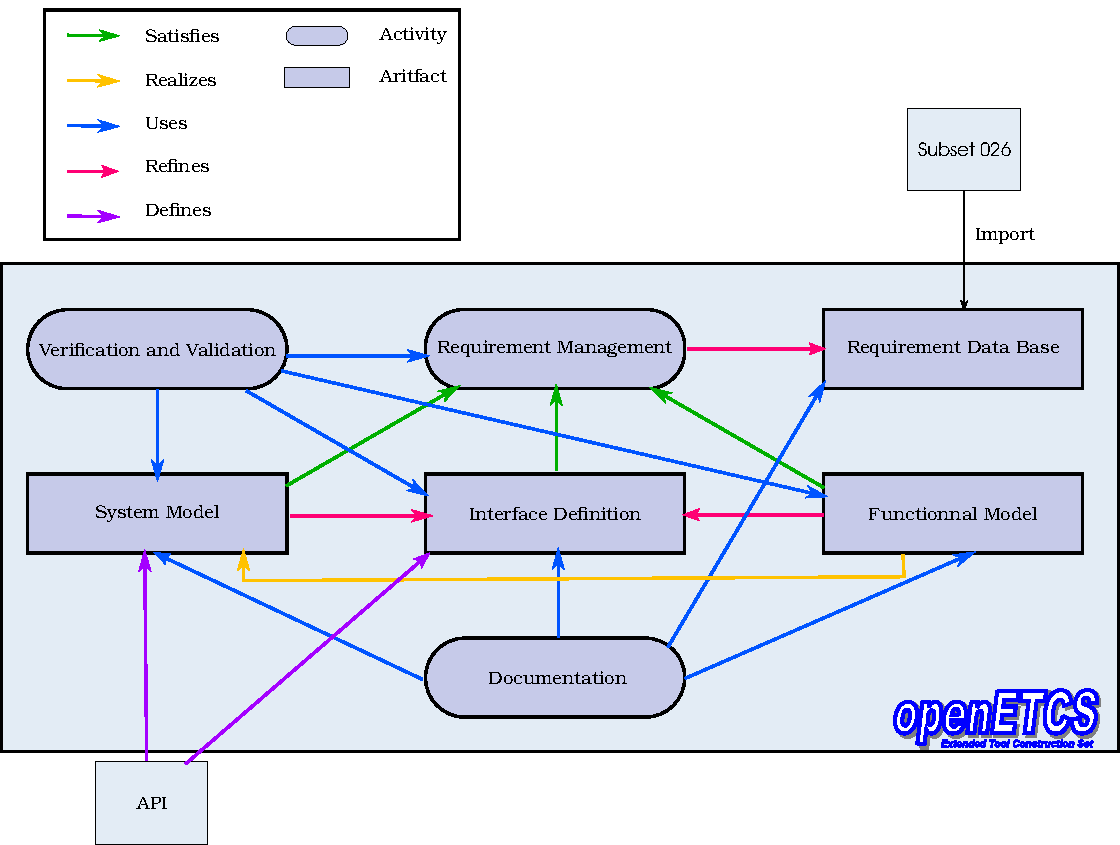
\includegraphics[width=.9\linewidth]{./images/trace_archi.pdf}
\caption{\label{fig:trace_process}Traceability architecture between artifacts}
\end{figure}

Figure  \ref{fig:trace_process} highlights the different artifacts or activities and their
links. Traceability activities should allow to trace a requirement within all
the artifacts and/or activities that are using it.

The goal of traceability is that, from any artifacts produced, we are able to
track which requirement it realizes, implements  or refers to. These links can
take different form and be done by different tools. 
Two traceability tools will be evaluate before being integrated in the OpenETCS tool chain:
ReqCycle and Reqtify.

The present solution proposes a first "by hand" approach, to deal with
traceability without having all the proper tools already integrated into the tool chain.

\section{First Solution}
\label{sec-1-1}
\begin{figure}[htb]
\centering
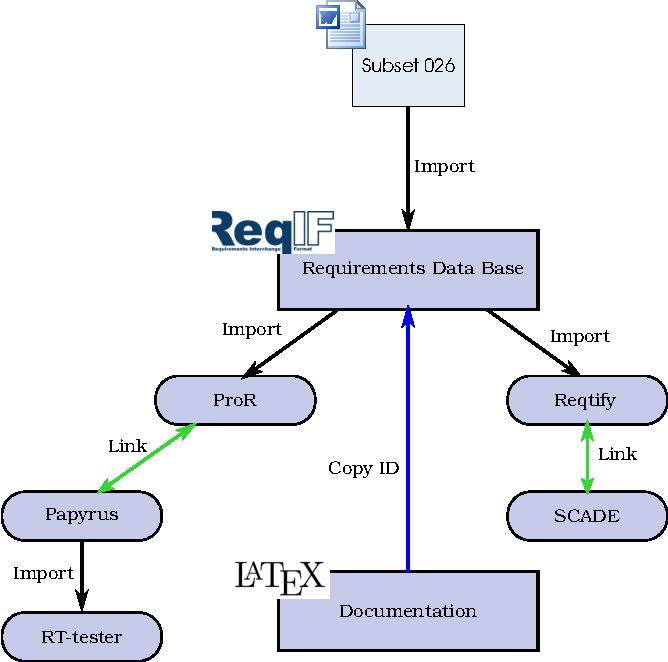
\includegraphics[width=.9\linewidth]{images/first_trace_solution.pdf}
\caption{\label{fig:trace_first}Traceability architecture first solution}
\end{figure}

Figure \ref{fig:trace_first} proposes a first solution to handle traceability.
The basic idea is to all refers to the same requirements data base. This data
base is itself directly imported from the subset-026 word document. The data
base provides the list of requirements as well as an unique identifiers for each
requirements. These identifiers are fixed and cannot be modified by any other
tools. But it may be possible for requirement management tools to refine these
requirements but they should guarantee the following rules:
\begin{enumerate}
\item The requirement's structure is not modified.
\item No requirement should be deleted.
\item Newly added requirements should be either refinement or a decomposition of an
existing one.
\item The identifier pattern should be respected.
\item Identifier should stay unique.
\end{enumerate}


\subsection{{\bfseries\sffamily TODO} ReqCycle  Evaluation}
\label{sec-1-2}
\subsection{{\bfseries\sffamily TODO} Reqtify Evaluation}
\label{sec-1-3}


\chapter{Activities Details}

\section{Subset-026 import}
\label{sec-2}
The subset-026 import is realized by a script transforming the Word document
into a req-IF format file.
\subsection{Script description}
\label{sec-2-1}
The script \todo{The script needs a name} generates a hierarchical tree of all traceworthy
artifacts in each chapter of subset-026. Each artifact shall be uniquely
addressable via a tracestring.


\subsection{Unique ID definition}
\label{sec-2-2}
Take the following example:
\begin{figure}[htb]
\centering
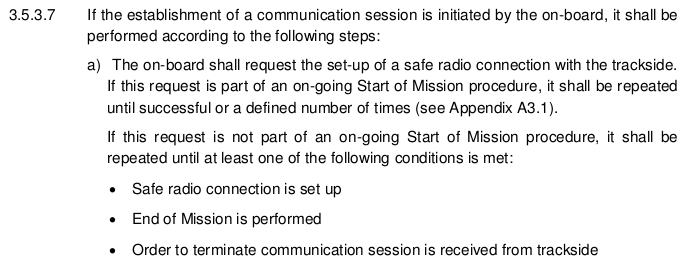
\includegraphics[width=.9\linewidth]{images/tracestring-ex.png}
\caption{\label{fig:reqID_ex}Traceability architecture between artifacts}
\end{figure}


\paragraph{Guideline}
The scope of a single requirement ID is a paragraph of text (there are six such
paragraphs in the above example).  requirement IDs are hierarchical. The
hierarchy is a direct mapping of the hierarchy in the original subset-026
text. Levels are separated by a dot. There is a requirement at each level
(i.e. you may truncate the requirement ID to any level and it stays valid).

\paragraph{How to}

Suppose we want to trace the fifth paragraph in the above example i.e
\begin{verbatim}
• End of mission is performed
\end{verbatim}
\begin{enumerate}
\item Let \textsl{traceString} be the variable to store the result.
\item Find the current running number of the base list. That is the list which
includes the chapter number. In this example this number equals
\verb+3.5.3.7.+ Set \textsl{traceString} to this number.
\item Count the number of paragraphs in this list item starting with 1 and append
this number in square brackets to the \textsl{traceString} if it is greater than 1.

Note: For the first iteration in the example there is only one such paragraph
(\texttt{If the establishment...}). Hence, we do not append anything. In the
second iteration there are two such paragraphs (\texttt{The on-board shall...} and
\texttt{If this request is not ...}). Hence, the second one will receive an
\texttt{[2]} appendix.

\item Until you arrived at your target paragraph: Append any running number of
sub-lists and remove leading or trailing characters (such as braces). If the
current sub-list is bulleted then the level string always becomes
\verb+[*][n]+ (with n being the running number of that bullet starting at
1). Prefix this new level with a dot (\verb+.+) and append it to the
\textsl{traceString}.

Note: \verb+a)+ is the identifier of one such sub-list item. The trailing brace
will be removed. The bullet points form another (less significant) sub-list.
\item Do step 3.
\item Do step 4 or break.
\item \textsl{traceString} is now the fully qualified requirementID.
\end{enumerate}

This will result in the following requirement ID: \quad \verb+3.5.3.7.a[2].[*][2]+


\section{Requirement Database}
\label{sec-3}
The requirement data base is a ReqIF file-based.

\section{Requirement management}
\label{sec-4}
The requirement management allows us to have a look at the set of requirements
and performs some actions.
The set of requirements can be automatically imported from a Req-IF file.

The requirement management should be use to refine the high-level requirements
from the import. It can be use to give more precise information about :
\begin{itemize}
\item Which requirements are implementable
\item Who is assigned to implement a set of requirements
\item How and if the requirement is decomposed.
\item TODO (list to be refined)
\end{itemize}

In the OpenETCS tool chain this tasks is done with ProR.
Alternatively to deal with the closed source path the requirement management may
be done by Reqtify Gateway of SCADE. 

\section{System Model}
\label{sec-5}

The system model defines block and interfaces between those blocks that realizes
the specification.
This is done with Papyrus. 

The link with the requirement may be included via requirements diagram with a
direct link of requirement in ProR
The explanation to performs the link may be found here \href{https://github.com/openETCS/toolchain/wiki/User-Documentation#tracing-requirements-and-sysml-models}{ProR-Papyrus proxy}.
The links may be viewed through Papyrus an ProR and the requirement may be
directly apply from ProR to a Papyrus elements.


\section{Interface Definition}
\label{sec-6}

Should define the interfaces between the architecture artifacts.  It is used and
set up to facilitate team working together on a big architecture. Its definition
comes from the requirements but can also be refines by the modeling team without
changing the existing implemented requirements.

\section{Functional model}
\label{sec-7}
The function model is the implementation of the system defines in the system
model. It should covers the set of implementable requirements.

\section{{\bfseries\sffamily TODO} Verification and Validation}
\label{sec-8}
% Emacs 24.3.1 (Org mode 8.2.4)
\end{document}

%%  LocalWords:  traceability OpenETCS
